% Section 3. Grounded rewrite 2026-11-03 (branch docs/cep-grounded-draft). Scale numbers: python -m optics.scale_chain
% (docs/optics/scale_chain.md); other numbers: scripts/rerun_paper_numbers.py --no-video (docs/optics/rerun_results.md).
% Claim changes: papers/cep/CLAIM_CHANGES.md.
\section{Geometric optics through the sight glass \emph{(RQ1)}}\label{sec:optics}

\subsection{Thin-lens scale model}\label{sec:thinlens}

Under the Gaussian thin-lens approximation \citep[\S\,5.2]{Hecht2017}, the object distance $d_o$ and the image
distance $i$ satisfy
\begin{equation}\label{eq:thinlens}
\frac{1}{f} = \frac{1}{d_o} + \frac{1}{i}, \qquad M = \frac{i}{d_o} = \frac{f}{d_o - f},
\end{equation}
with $M$ the transverse magnification. An extension tube of length $e$ sets the image distance at infinity focus
to $f + e$ \citep{PhotonsToPhotos2024}, and the focus helicoid adds its travel $x$, so that
$i = f + e + x = 96$~mm and the focused object distance is $d_\mathrm{focus} = f i / (i - f) = 55.08$~mm, with
$M = 1.743$ (\tabref{tab:inputs}; \code{scripts/rerun_paper_numbers.py}). Once focus is set, $i$ is fixed. A point
at lateral position $X$ and depth $d_o$ is imaged, sharp or blurred, about the chief ray through the lens centre,
at $X i / d_o$ on the sensor. The object-plane extent of one recorded pixel of sensor-plane pitch $p_k$ along axis
$k \in \{x, y\}$ is therefore
\begin{equation}\label{eq:pixelsize}
\Delta_k(d_o) = \frac{p_k}{M(d_o)} = p_k \, \frac{d_o}{i},
\end{equation}
linear in $d_o$ (\figref{fig:mmpx}), with the pitches $p_x \neq p_y$ of the signal chain (\secref{sec:chain}). At
the focused plane $\Delta_k = p_k f / (e + x)$, so the scale there depends only on $f$, $e$ and
$x$.

\begin{figure}
\centering
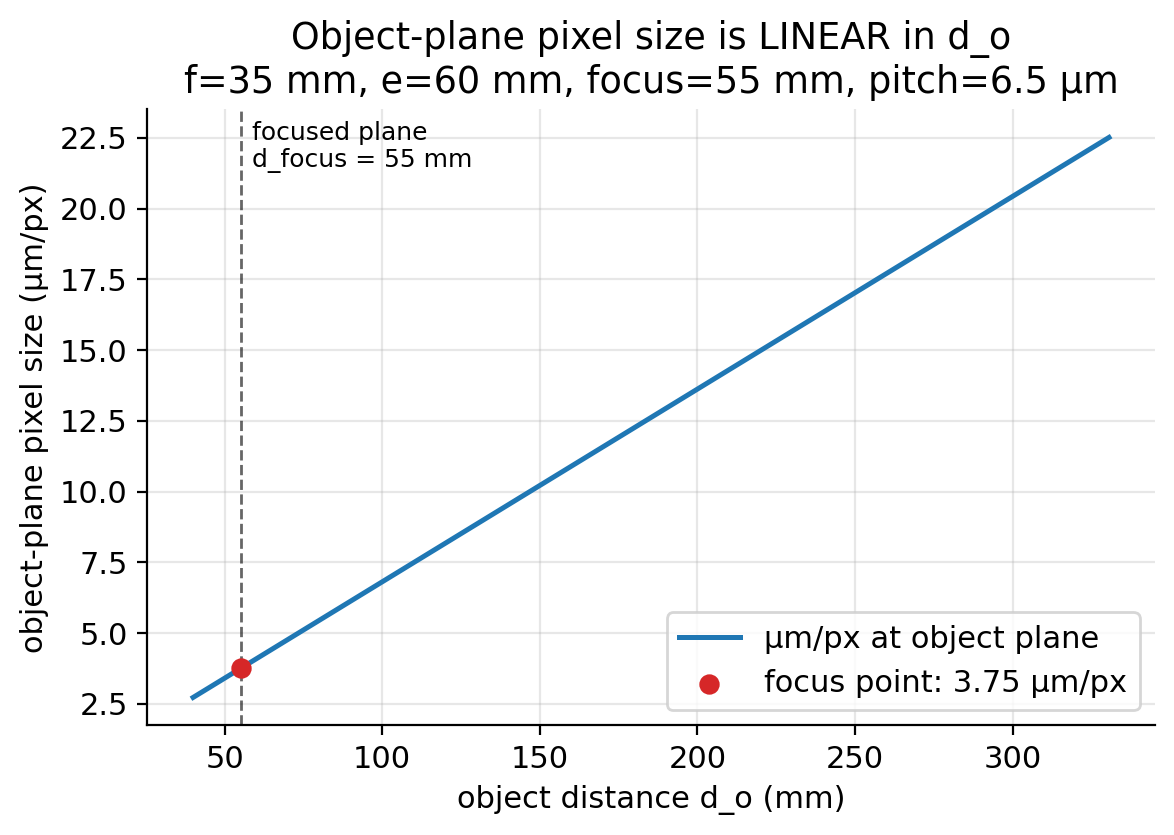
\includegraphics[width=\columnwidth]{01_mm_per_pixel}
\caption{\textbf{How does the metric scale change with depth?} Object-plane extent of one PAL sample, taken as the
geometric mean of its two axes (6.53~\um{} on the sensor), against object distance for $f = 35$~mm, $e = 60$~mm and
$x = 1$~mm. The curve is linear in $d_o$ (Eq.~\ref{eq:pixelsize}); at the focused plane it is 3.75~\umpx. The
per-axis values are given in \tabref{tab:scale}.}\label{fig:mmpx}
\end{figure}

\subsection{Pixel scale at the focused plane and its uncertainty}\label{sec:budget}

\tabref{tab:scale} gives the per-axis scale of both recording types at the focused plane
(\code{python -m optics.scale_chain}; \code{docs/optics/scale_chain.md}). The uncertainty comes from a Monte Carlo
propagation over 200\,000 draws of the inputs of \tabref{tab:inputs}: $e$ uniform within $\pm 5$~mm (the plant's
``$\approx 6$~cm'' read as rounded to the centimetre), $x$ uniform over 0--2~mm, $f$ normal with $\sigma = 2$\,\%
(assumed lens tolerance), the line-to-sample mapping uniform within $\pm 2$\,\% (x only), the camera candidate
(x up to $+0.6$\,\%, y up to $+0.8$\,\%) and the measured 1080p stretch ($\pm 0.1$\,\%). Every entry is an estimate:
it inherits the approximate tube length and the unconfirmed camera model.

\begin{table}
\centering\tabfont
\caption{Object-plane pixel scale at the focused plane, \umpx{} (median and 95\,\% interval of the Monte Carlo
budget; nominal in brackets). Last column: the same if the stated tube length includes a 5~mm CS-to-C ring.
Source: \texttt{python -m optics.scale\_chain}.}\label{tab:scale}
\begin{tabular}{@{}llrrr@{}}
\toprule
Recording & Axis & Median [nominal] & 95\,\% interval & With ring \\
\midrule
PAL $720 \times 576$ & x & 3.932 [3.919] & 3.576--4.347 & 4.283 \\
PAL $720 \times 576$ & y & 3.601 [3.586] & 3.285--3.967 & 3.923 \\
1080p clip & x & 1.469 [1.464] & 1.336--1.624 & 1.600 \\
1080p clip & y & 1.921 [1.913] & 1.752--2.116 & 2.092 \\
\bottomrule
\end{tabular}
\end{table}

The 95\,\% interval is about $\pm 10$\,\% on either axis ($\pm 9.8$\,\% along x, $\pm 9.5$\,\% along y), and the
tube length dominates it: $e \pm 5$~mm alone moves the scale by $-7.6$ to $+8.9$\,\%, against $\pm 2.0$\,\% for the
focal-length tolerance, $\pm 2.0$\,\% for the line mapping, $-1.6$ to $+1.7$\,\% for the focus travel and less than
1\,\% for the camera candidate. Whether a 5~mm CS-to-C ring is counted in the 60~mm is a discrete alternative,
$+8.9$\,\%, kept outside the interval. The glass index, the glass thickness and the air gap do not enter: a
parallel plate moves the focused plane but leaves the magnification at a fixed $i$ unchanged. A caliper reading of
$e$ and a photograph of the mount would remove the two largest terms.

For sizes, the per-axis scale matters. A clip pixel is 1.464~\um{} wide and 1.913~\um{} tall in the slurry, so a
length measured along a row is 12\,\% shorter and one measured down a column 15\,\% longer than with the
geometric-mean pixel of 1.673~\um, which is appropriate only for areas. The geometric mean of the PAL sample is
3.749~\um; a PAL sample, not a clip pixel, is the resolution element of both recordings (\secref{sec:chain}).

\subsection{Sight-glass refractive shift}\label{sec:shift}

A parallel plate of thickness $t$ and index $n_g$ shifts the apparent object distance toward the lens by
$\Delta = t (1 - 1/n_g)$ in the paraxial limit \citep{Hecht2017}. For $t = 20$~mm and the assumed $n_g = 1.47$,
$\Delta = 6.39$~mm, independent of distance; $n_g = 1.52$ would give 6.84~mm (\figref{fig:shift};
\code{scripts/rerun_paper_numbers.py}). The shift moves the focused plane relative to the glass but, as stated
above, not the scale. The exact projection through a flat port is of high polynomial degree (12th degree for two
refractions with distinct indices, \citealp{Agrawal2012}); we use the paraxial form and have not computed the
residual distortion over the field.

\begin{figure}
\centering
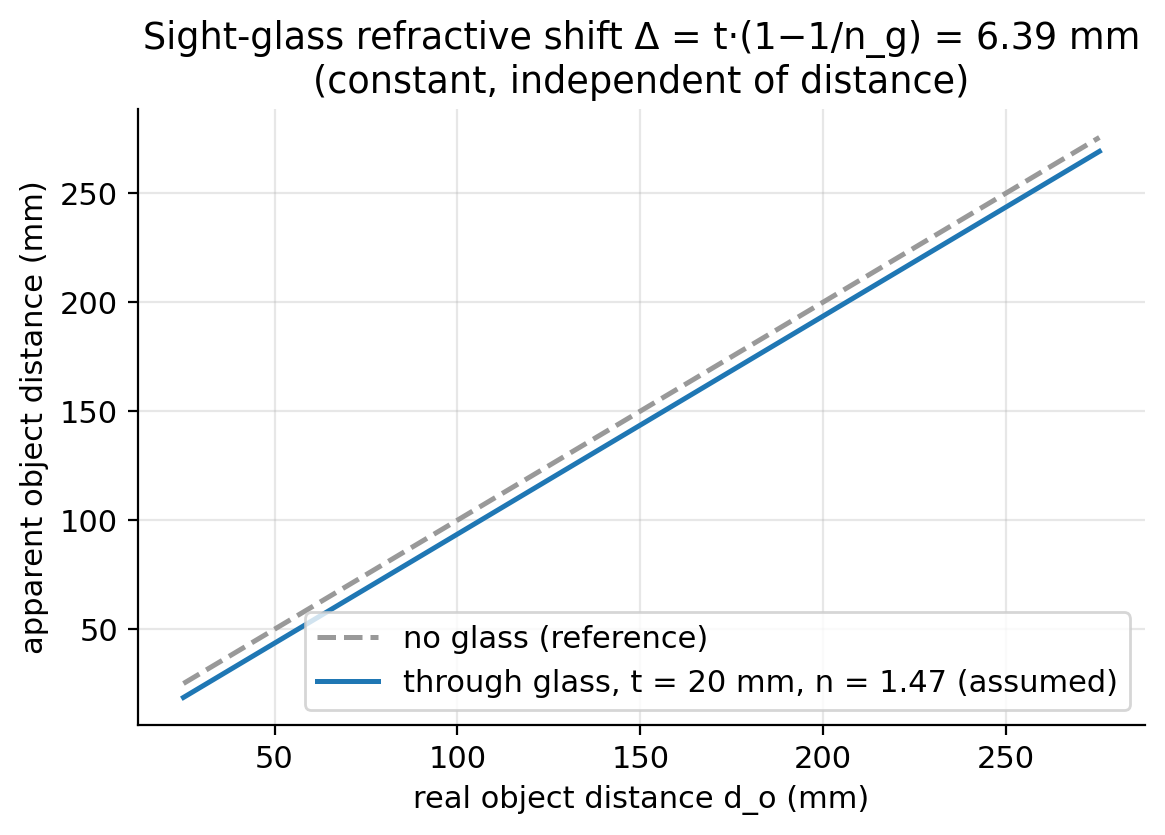
\includegraphics[width=\columnwidth]{05_sight_glass_shift}
\caption{\textbf{How much does the sight glass move the object?} Apparent against real object distance through a
20~mm plate of assumed index $n_g = 1.47$. The paraxial shift is a constant $\Delta = 6.39$~mm; it offsets every
$d_o$ but does not change the slope of \figref{fig:mmpx}.}\label{fig:shift}
\end{figure}

\subsection{Extension-tube sensitivity}\label{sec:tube}

At the focused plane the scale is proportional to $1/(e + x)$ (\secref{sec:thinlens}), so the tube length acts as a
multiplicative factor on every reported size: each $\pm 1$~mm of $e$ or of focus travel moves the scale by
$\mp 1.64$\,\%. \figref{fig:tube} shows the consequence over a standard extension-ring set. A 10~mm tube instead of
60~mm would make the scale 5.55 times coarser, $8.12 \times 10.61$~\umpx{} on a clip pixel.

The tube length cannot be recovered reliably from the image by anchoring a typical crystal size, because that size
changes by more than an order of magnitude within a strike (the microscope medians of \secref{sec:plant} grow from
29 to 483~\um{} in two hours). A wrong tube length would rescale the whole distribution without making it
internally inconsistent. The tube must therefore be measured; in the absence of a caliper reading the plant's
``$\approx 6$~cm'' leaves the $\pm 10$\,\% interval of \tabref{tab:scale}.

\begin{figure}
\centering
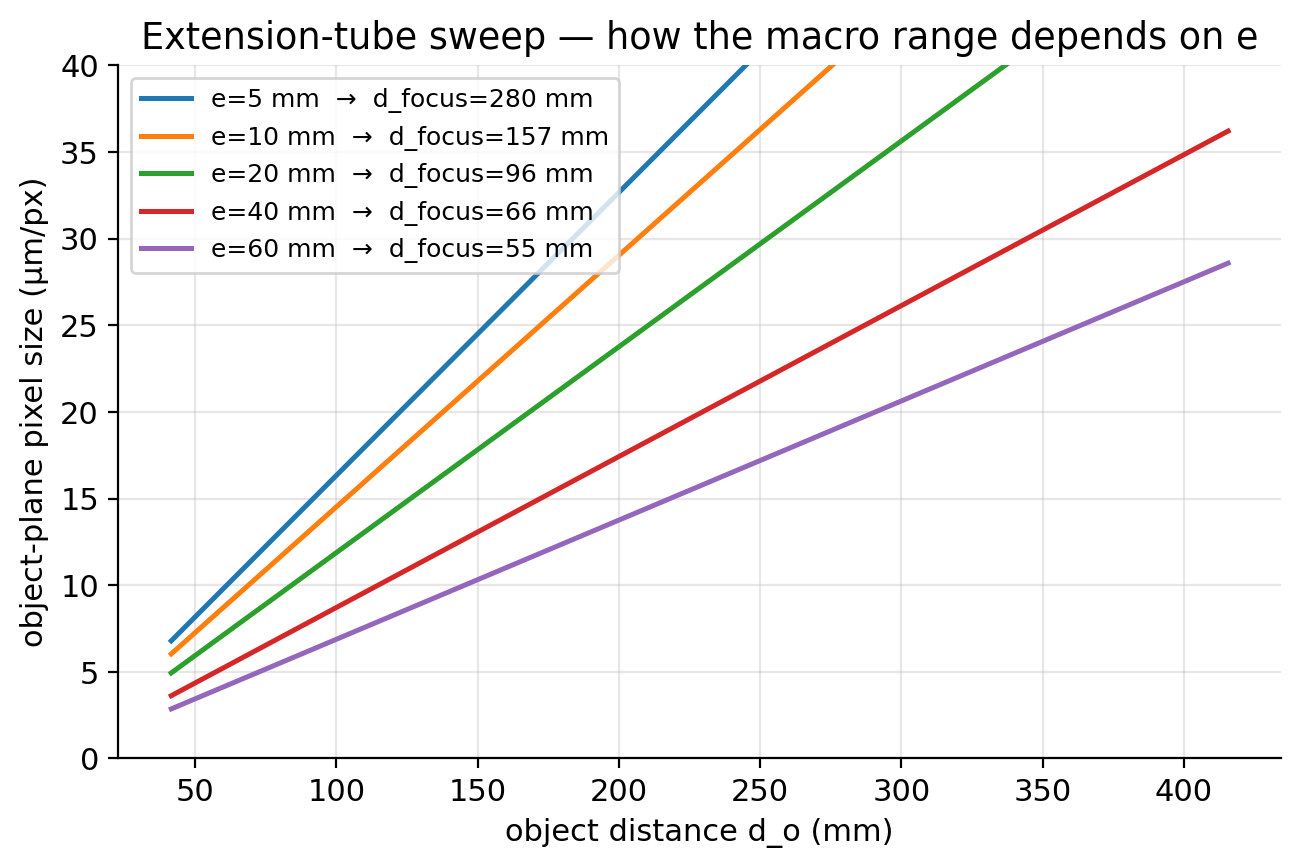
\includegraphics[width=\columnwidth]{06_extension_tube_sweep}
\caption{\textbf{How does the extension tube set the macro range?} Object-plane extent of the geometric-mean PAL
sample against object distance for tube lengths of 5, 10, 20 and 40~mm (an analysis choice) and the installed
${\approx}\,60$~mm. The legend gives the focused distance of each tube; the curves are drawn without the focus
travel, $i = f + e$.}\label{fig:tube}
\end{figure}

\subsection{Where the focal plane sits relative to the glass}\label{sec:slab}

\figref{fig:layout} draws the optical stack to scale. The lens datasheet gives the back focal distance but not the
position of the front principal plane $H$ \citep{FujinonHF35HA1B}, so the focused plane cannot be placed
relative to the glass from the datasheet and the plant geometry alone. The geometry is, however, consistent with a
focal plane at the inner glass face. In that case the real distance from $H$ to the inner face is
$d_\mathrm{focus} + \Delta = 55.08 + 6.39 = 61.47$~mm, and subtracting $t = 20$~mm and $a \approx 20$~mm places $H$
$21.5 \pm 3.4$~mm (1$\sigma$, \code{python -m optics.error_budget}) behind the front element, inside the 30.5~mm lens body (29.5~mm plus the 1~mm focus travel). On the image
side, for a C-mount body, the flange depth of 17.53~mm, the tube and the lens body put the rear principal plane $H'$, which lies
$i = 96$~mm in front of the sensor, 12.0~mm behind the front element (\code{python -m optics.error_budget}). Both
planes then fall inside the lens body. This is a consistency check on the stated geometry, not a measurement of the
focal-plane position. An empty-tank frame in which the scratches of the glass's inner face are sharp would locate
the plane directly.

\begin{figure*}
\centering
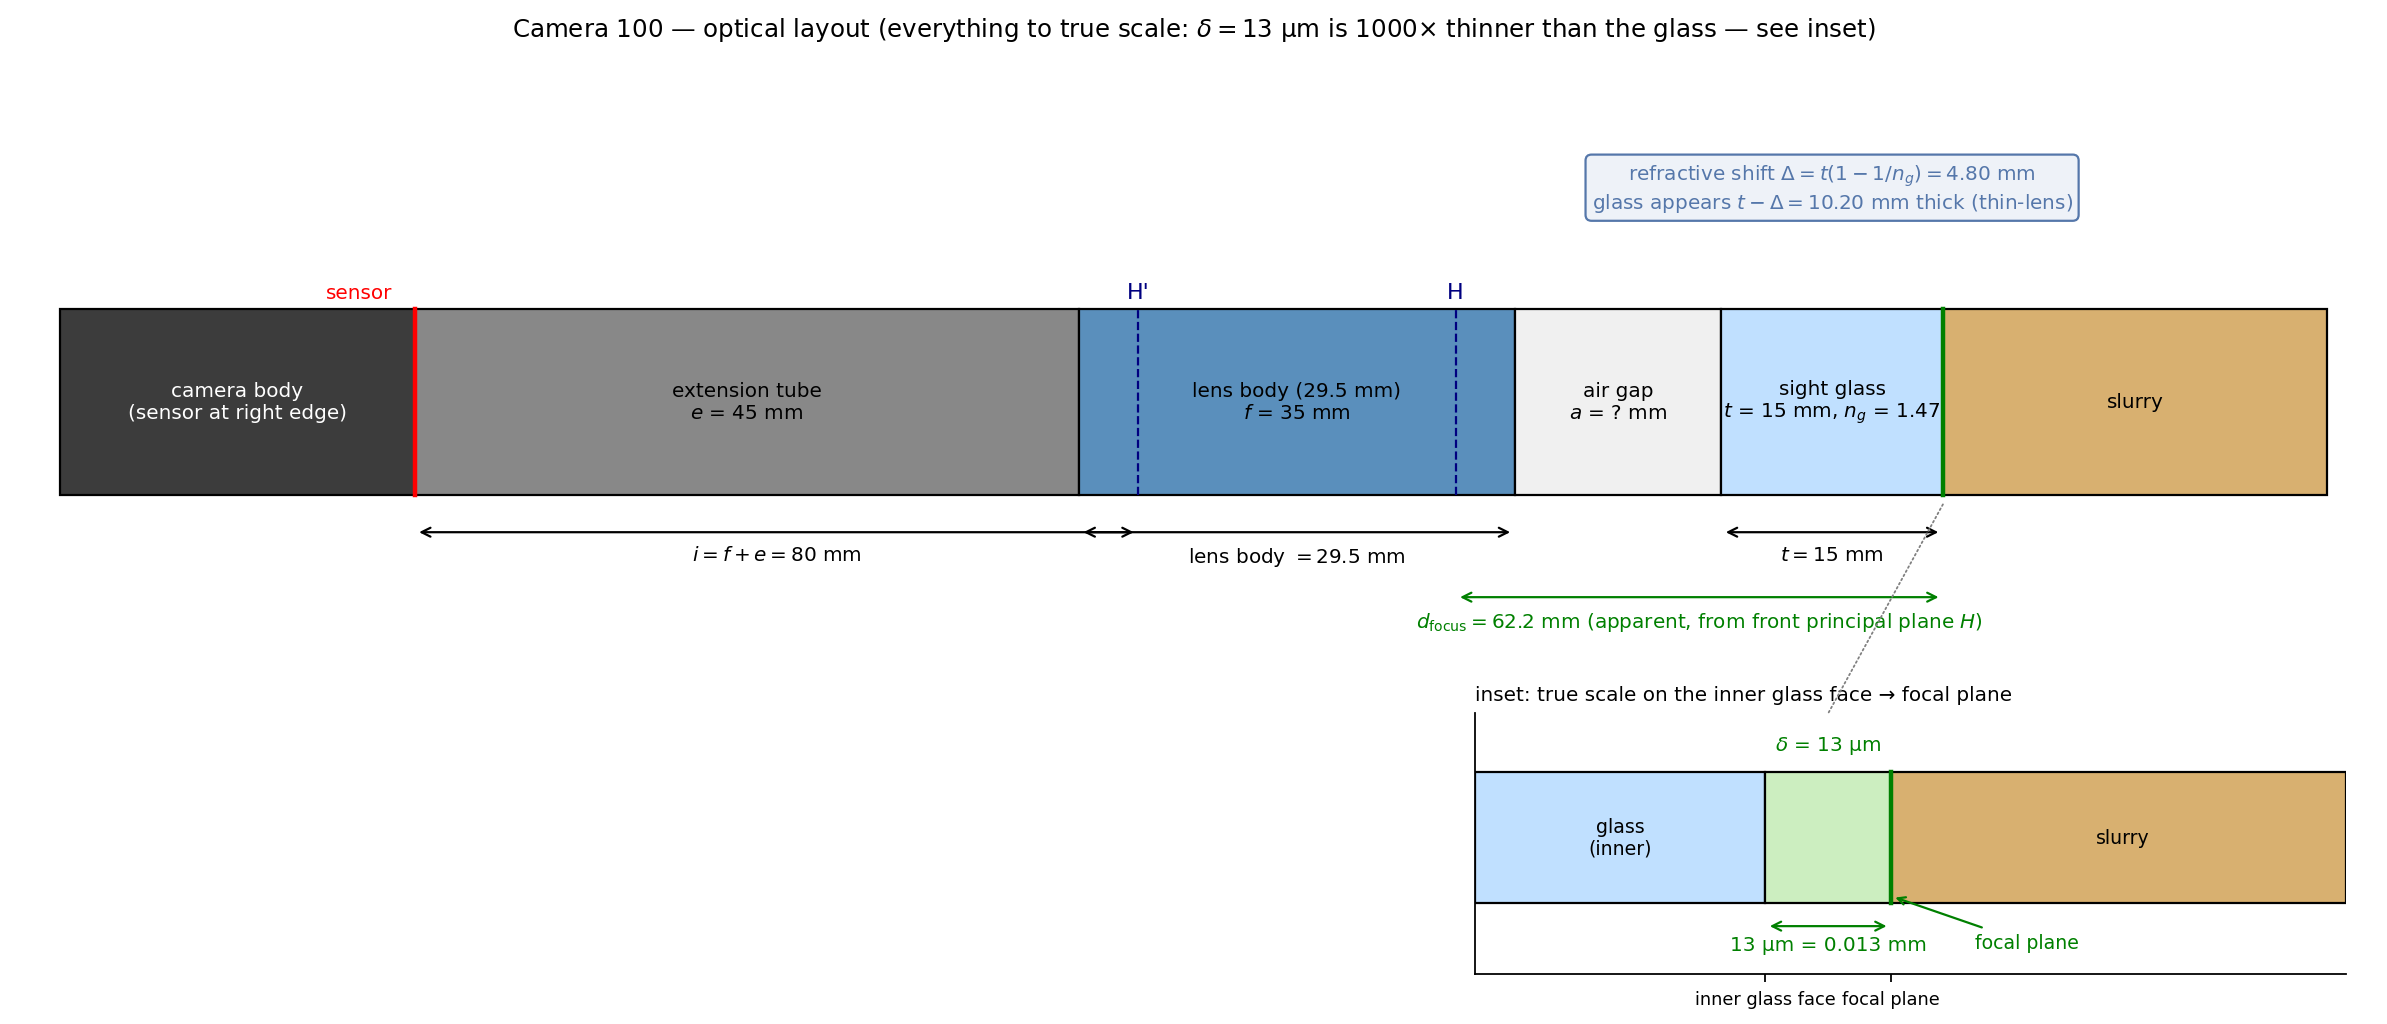
\includegraphics[width=0.85\textwidth]{18_optical_layout}
\caption{\textbf{What does the optical chain from sensor to slurry look like?} Layout drawn to scale from
\texttt{configs/camera\_100.toml} (\texttt{python -m optics.optical\_layout}); the colour of each dimension gives its
source class. Camera body length (40~mm) and lens body (30.5~mm, including the 1~mm focus travel) are estimates;
tube $e$, air gap $a$ and glass $t$ are plant statements; the sensor-to-$H'$ distance $i = f + e + x = 96$~mm is
derived. The placement of the sharp-focus plane at the inner glass face, and hence $H \to$ focus $= 61.5$~mm, is an
assumption (\secref{sec:slab}).}\label{fig:layout}
\end{figure*}

If the focal plane does lie at the inner glass face, the camera samples the slurry layer pressed against the glass,
with an in-focus slice of $\pm 9.4$~\um{} (\secref{sec:dof}). That this layer represents the bulk of the stirred
pan is the homogeneity assumption of \secref{sec:homog}, not a measured fact. The vessel dimensions play no role in
the depth range: the optical slice is far thinner than any vessel dimension.
